% LaTex Compiler

\documentclass[10pt]{article}
\usepackage[usenames]{color} %used for font color
\usepackage{amssymb} %maths
\usepackage{amsmath} %maths
\usepackage[utf8]{inputenc} %useful to type directly diacritic characters
\usepackage{tikz-feynman}

\begin{document}

\textbf{\textcolor{blue}{An example: one loop bubble diagram and its IBP relations}}

Let us consider the following integral
\begin{eqnarray}
\nonumber
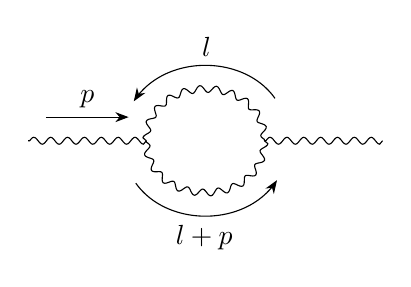
\begin{tikzpicture}
\begin{feynman}
  \vertex (a);
  \vertex [right=of a](b);
  \vertex [right=of b](c);
  \vertex [right=of c](d);
  
  \diagram* {
    (a) -- [boson, momentum=\(p\)] (b),
    (c) -- [boson] (d),
    (c) -- [boson, half right, momentum'=\(l\)] (b),
    (b) -- [boson, half right, momentum'=\(l+p\)] (c),
  };
\end{feynman}
\end{tikzpicture}
\end{eqnarray}
where we consider general powers on denominators:
\begin{align*}
I(n_1,n_2) &= \int d^d l_1 d^d l_2 \frac{1}{D_1^{n_1} D_2^{n_2}} \\
D_1 &:= l^2 \\
D_2 &:= (l+p)^2.
\end{align*}

Consider an IBP relation generated by
\begin{align}
\nonumber
\frac{\partial}{\partial l} \cdot p \frac{1}{D_1^{n_1} D_2^{n_2}}
&=
\frac{-n_1}{D_1^{n_1+1}} p \cdot \frac{\partial D_1}{\partial l} \frac{1}{D_2^{n_2}}
+
\frac{1}{D_1^{n_1}} \frac{-n_2}{D_2^{n_2+1}} p \cdot \frac{\partial D_2}{\partial l} \\
\nonumber
&=
\frac{-n_1 2p\cdot l}{D_1^{n_1+1} D_2^{n_2}}
+
\frac{-n_2 p\cdot (2p+2l)}{D_1^{n_1} D_2^{n_2+1}}
\end{align}
Since $p^2$ is an "external" parameter of this event, and
\begin{equation}
\nonumber
D_2 - D_1 - p^2 = 2p\cdot l
\end{equation}
implies that
\begin{align}
\nonumber
rhs&=
\frac{-n_1 ( D_2 - D_1 - p^2 )}{D_1^{n_1+1} D_2^{n_2}}
+
\frac{-n_2p\cdot (2p^2+ D_2 - D_1 - p^2)}{D_1^{n_1} D_2^{n_2+1}}\\
\nonumber
&=
\frac{n_1-n_2}{D_1^{n_1} D_2^{n_2}} 
+ \frac{n_1p^2}{D_1^{n_1+1} D_2^{n_2}}
+ \frac{-n_2p^2}{D_1^{n_1} D_2^{n_2+1}}
+ \frac{n_2}{D_1^{n_1-1} D_2^{n_2+1}}
+ \frac{-n_1}{D_1^{n_1+1} D_2^{n_2-1}}
\end{align}
and we get a linear equation
\begin{align}
\nonumber
0 &= (n_1-n_2) I(n_1,n_2) + n_1p^2 I(n_1+1, n_2) + (-n_2p^2) I(n_1,n_2+1) \\
\nonumber
   &+ n_2I(n_1-1,n_2+1) + (-n_1)I(n_1+1, n+2-1)
\end{align}

Similarly, we can take 
\begin{equation}
\nonumber
\frac{\partial}{\partial l} \cdot \frac{l}{D_1^{n_1} D_2^{n_2}}
= 
\frac{\partial l}{\partial l} \frac{1}{D_1^{n_1} D_2^{n_2}}
+
l\cdot
\frac{\partial}{\partial l} \frac{1}{D_1^{n_1} D_2^{n_2}}
=
d \frac{1}{D_1^{n_1} D_2^{n_2}}
+
l\cdot
\frac{\partial}{\partial l} \frac{1}{D_1^{n_1} D_2^{n_2}}
\end{equation}
and get another linear relation
\begin{equation}
\nonumber
0 = (d-n_1 -2n_2)I(n_1,n_2) + (-n_2) I((n_1-1, n_2+1) + n_1 p^2 I(n_1, n_2+1) 
\end{equation}
If we restrict $0 < n_1, n_2$ then with these equations, we can reduce any indices into $(1,1)$.
Thus, any integral is written as a product of some rational function of $d, n_1,n_2$ and $I(1,1)$, where $I(1,1)$ is called a Master Integral of this system.

\end{document}
